\documentclass[border=2mm]{standalone}

\usepackage{tikz}
\usetikzlibrary{shapes,snakes}
\usepackage{amsmath,amssymb,fontawesome}
\usepackage{xcolor}
\usetikzlibrary{decorations.pathreplacing,positioning, arrows.meta}

\definecolor{pink}{RGB}{205, 125, 169}
\definecolor{blue}{RGB}{36, 118, 182}
\definecolor{orange}{RGB}{230, 160, 46}
\definecolor{green}{RGB}{71, 159, 119}

%	\textcolor{orange}{\faSquare} HMD-Liv %
%	\textcolor{pink}{\faSquare} HMD-Pyr %
%	\textcolor{blue}{\faSquare} DT-Liv %
%	\textcolor{green}{\faSquare} DT-Pyr % 

\newcommand{\ImageWidth}{7cm}

\begin{document}



% Define box and box title style
\tikzstyle{mybox} = [draw=black, fill=white, very thick,
    rectangle, rounded corners, inner sep=10pt, inner ysep=11pt]
\tikzstyle{fancytitle} =[fill=black, text=white, rounded corners]

%\begin{tikzpicture}
%\node[draw,text width=3cm] at (0,2) { \tiny 
%\textcolor{orange}{\faSquare} HMD-Liv \textcolor{pink}{\faSquare} HMD-Pyr \textcolor{blue}{\faSquare} DT-Liv \textcolor{green}{\faSquare} DT-Pyr % 
%};
%\end{tikzpicture}

\begin{tikzpicture}
%\node[text width=4cm] at (0, 3) {\small \begin{flushleft}\bf User groups\end{flushleft}};
%\node[text width=7cm] at (3,2) { \tiny
%\textcolor{orange}{\faSquare} HMD-Liv \thinspace\thinspace \textcolor{blue}{\faSquare} DT-Liv \textcolor{pink}{\faSquare} HMD-Pyr \thinspace \textcolor{green}{\faSquare} DT-Pyr};

%\node[black, align=center, font=\scriptsize] at (-.5, 0) {\textcolor{orange}{\faSquare}};

\node[text width=5pt, left=7pt] at (0,.71) { \scriptsize \textcolor{orange}{\faSquare} };
\node[text width=5pt, left=7pt] at (0,.351) { \scriptsize \textcolor{blue}{\faSquare} };
%\node[text width=5pt, left=2pt] at (0,-.71) { \scriptsize \textcolor{pink}{\faSquare} };
%\node[text width=5pt, left=2pt] at (0,.-1.151) { \scriptsize \textcolor{green}{\faSquare} };

% draw horizontal line   
\draw[thick, -Triangle] (0,0) -- (\ImageWidth,0) node[font=\scriptsize,below left=3pt and -8pt]{sub-steps};

% draw vertical lines
\foreach \x in {0,1,...,6}
\draw (\x cm,3pt) -- (\x cm,-3pt);

%\foreach \x/\descr in {1/Interaction, 5/t-1,6/t,7/t+1}
%\node[font=\scriptsize, text height=1.75ex,
%text depth=.5ex] at (\x,-.3) {\descr};

% colored bar above (liver)

\foreach \x/\perccol in {2/0, 3/0, 4/0, 5/0} \draw[lightgray!\perccol!lightgray, line width=5pt] (\x,.35) -- +(1,0);
\foreach \x/\perccol in {2/0, 3/0, 4/0, 5/0} \draw[lightgray!\perccol!lightgray, line width=5pt] (\x,.7) -- +(1,0);

%\foreach \x/\perccol in {2/0, 3/0, 4/0, 5/0} \draw[lightgray!\perccol!orange, line width=5pt] (\x,.7) -- +(.9,0);
%\foreach \x/\perccol in {2/0, 3/0, 4/0, 5/0} \draw[lightgray!\perccol!blue, line width=5pt] (\x,.7) -- +(.75,0);
%\foreach \x/\perccol in {2/0, 3/0, 4/0, 5/0} \draw[lightgray!\perccol!orange, line width=5pt] (\x,.7) -- +(.6,0);
%\foreach \x/\perccol in {2/0, 3/0, 4/0, 5/0} \draw[lightgray!\perccol!blue, line width=5pt] (\x,.7) -- +(.45,0);
%\foreach \x/\perccol in {2/0, 3/0, 4/0, 5/0} \draw[lightgray!\perccol!orange, line width=5pt] (\x,.7) -- +(.3,0);
%\foreach \x/\perccol in {2/0, 3/0, 4/0, 5/0} \draw[lightgray!\perccol!blue, line width=5pt] (\x,.7) -- +(.15,0);

\foreach \x/\perccol in {0/0, 1/0} 
% {1/25, 2/0, 3/0, 4/0, 5/0} % 1/75, 2/25, 3/0
\draw[lightgray!\perccol!orange, line width=5pt] 
(\x,.7) -- +(1,0);
\draw[-Triangle, dashed, thick, orange] (6,.7) --  +(1,0);
\foreach \x/\perccol in {2/100} \draw[white, line width=6pt] (\x,.7) -- +(0.3,0);

\foreach \x/\perccol in {0/0, 1/0} 
\draw[lightgray!\perccol!blue, line width=5pt] 
(\x,.35) -- +(1,0);
\draw[-Triangle, dashed, thick, blue] (6,.35) --  +(1,0);
\foreach \x/\perccol in {2/100} \draw[white, line width=6pt] (\x,.35) -- +(0.3,0);

%% colored bar below (pyramid)
%\foreach \x/\perccol in
%{1/25, 2/0, 3/0, 4/0, 5/0} % 1/75, 2/25, 3/0
%\draw[lightgray!\perccol!pink, line width=5pt] 
%(\x,-.7) -- +(1,0);
%\draw[-Triangle, dashed, thick, pink] (6,-.7) --  +(1,0);
%\foreach \x/\perccol in {2/100} \draw[white, line width=6pt] (\x,-.7) -- +(0.3,0);
%
%\foreach \x/\perccol in
%{1/25, 2/0, 3/0, 4/0, 5/0} % 1/75, 2/25, 3/0
%\draw[lightgray!\perccol!green, line width=5pt] 
%(\x,-1.15) -- +(1,0);
%\draw[-Triangle, dashed, thick, green] (6,-1.15) --  +(1,0);
%\foreach \x/\perccol in {2/100} \draw[white, line width=6pt] (\x,-1.15) -- +(0.3,0);

% horizontal braces
%\draw [decorate, decoration={brace,amplitude=5pt}] (1,1.15)  -- +(1,0)
%	node [black, midway, above=4pt, font=\scriptsize] {Condition};
\draw [decorate, decoration={brace,amplitude=4pt}] (0,1.15)  -- +(2,0)
	node [black, midway, above=4pt, font=\scriptsize] {Interaction};
%\draw [decorate,decoration={brace,amplitude=4pt}] (2,1.35)  -- +(2,0) 
%       node [black,midway,above=4pt, font=\scriptsize] {Task 1};
\draw [decorate,decoration={brace,amplitude=4pt}] (4,1.15)  -- +(2,0) 
       node [black,midway,above=4pt, font=\scriptsize] {Task 2};

\draw[decorate,decoration={brace,amplitude=4pt}] (4,-0.3) -- (2,-0.3)
    node[anchor=north,midway,below=4pt] {\scriptsize Task 1};
%\draw[decorate,decoration={brace,amplitude=4pt}] (6,-0.3) -- (2.3,-0.3)
%    node[anchor=north,midway,below=4pt] {\scriptsize Common for Liv groups};

% vertical braces
\draw [decorate,decoration={brace,amplitude=4pt},xshift=0.5pt,yshift=0pt]
      (-.8,.15) -- (-.8,.9) node [align=center,midway,left,xshift=-4pt] {\scriptsize Liv};
%\draw [decorate,decoration={brace,amplitude=4pt},xshift=0.5pt,yshift=0pt]
%      (-.5,-1.4) -- (-.5,-.5) node [midway,left,xshift=-5pt] {\scriptsize Pyr};
      
% annotations
\draw[blue,dashed,thick,decorate,decoration={brace,amplitude=0pt}] (1,.35) -- (-0.4,.35);
\draw[blue,dashed,thick,decorate,decoration={brace,amplitude=0pt}] (2.3,.35) -- (2,.35);
\draw[orange,dashed,thick,decorate,decoration={brace,amplitude=0pt}] (1,.7) -- (-0.4,.7);
\draw[orange,dashed,thick,decorate,decoration={brace,amplitude=0pt}] (2.3,.7) -- (2,.7);
%
%\draw[pink,dashed,thick,decorate,decoration={brace,amplitude=0pt}] (1,-.7) -- (0,-.7);
%\draw[pink,dashed,thick,decorate,decoration={brace,amplitude=0pt}] (2.3,-.7) -- (2,-.7);
%\draw[green,dashed,thick,decorate,decoration={brace,amplitude=0pt}] (1,-1.15) -- (0,-1.15);
%\draw[green,dashed,thick,decorate,decoration={brace,amplitude=0pt}] (2.3,-1.15) -- (2,-1.15);


%% test steps
%\draw [thick,decorate,decoration={brace,amplitude=0pt}] (4,-.2) -- +(-1,0);
%\draw [thick,decorate,decoration={brace,amplitude=0pt}] (4,-.25) -- +(-1,0);
%\draw [thick,decorate,decoration={brace,amplitude=0pt}] (6,-.2) -- +(-1,0);
%\draw [thick,decorate,decoration={brace,amplitude=0pt}] (6,-.25) -- +(-1,0);

% steps
%\node[black, align=center, font=\scriptsize] at (4.5,-0.3) {train};

\end{tikzpicture}

\end{document}